% Template for PLoS
% Version 3.1 February 2015
%
% To compile to pdf, run:
% latex plos.template
% bibtex plos.template
% latex plos.template
% latex plos.template
% dvipdf plos.template
%
% % % % % % % % % % % % % % % % % % % % % %
%
% -- IMPORTANT NOTE
%
% This template contains comments intended 
% to minimize problems and delays during our production 
% process. Please follow the template instructions
% whenever possible.
%
% % % % % % % % % % % % % % % % % % % % % % % 
%
% Once your paper is accepted for publication, 
% PLEASE REMOVE ALL TRACKED CHANGES in this file and leave only
% the final text of your manuscript.
%
% There are no restrictions on package use within the LaTeX files except that 
% no packages listed in the template may be deleted.
%
% Please do not include colors or graphics in the text.
%
% Please do not create a heading level below \subsection. For 3rd level headings, use \paragraph{}.
%
% % % % % % % % % % % % % % % % % % % % % % %
%
% -- FIGURES AND TABLES
%
% Please include tables/figure captions directly after the paragraph where they are first cited in the text.
%
% DO NOT INCLUDE GRAPHICS IN YOUR MANUSCRIPT
% - Figures should be uploaded separately from your manuscript file. 
% - Figures generated using LaTeX should be extracted and removed from the PDF before submission. 
% - Figures containing multiple panels/subfigures must be combined into one image file before submission.
% For figure citations, please use "Fig." instead of "Figure".
% See http://www.plosone.org/static/figureGuidelines for PLOS figure guidelines.
%
% Tables should be cell-based and may not contain:
% - tabs/spacing/line breaks within cells to alter layout or alignment
% - vertically-merged cells (no tabular environments within tabular environments, do not use \multirow)
% - colors, shading, or graphic objects
% See http://www.plosone.org/static/figureGuidelines#tables for table guidelines.
%
% For tables that exceed the width of the text column, use the adjustwidth environment as illustrated in the example table in text below.
%
% % % % % % % % % % % % % % % % % % % % % % % %
%
% -- EQUATIONS, MATH SYMBOLS, SUBSCRIPTS, AND SUPERSCRIPTS
%
% IMPORTANT
% Below are a few tips to help format your equations and other special characters according to our specifications. For more tips to help reduce the possibility of formatting errors during conversion, please see our LaTeX guidelines at http://www.plosone.org/static/latexGuidelines
%
% Please be sure to include all portions of an equation in the math environment.
%
% Do not include text that is not math in the math environment. For example, CO2 will be CO\textsubscript{2}.
%
% Please add line breaks to long display equations when possible in order to fit size of the column. 
%
% For inline equations, please do not include punctuation (commas, etc) within the math environment unless this is part of the equation.
%
% % % % % % % % % % % % % % % % % % % % % % % % 
%
% Please contact latex@plos.org with any questions.
%
% % % % % % % % % % % % % % % % % % % % % % % %

\documentclass[10pt,letterpaper]{article}
\usepackage[top=0.85in,left=2.75in,footskip=0.75in]{geometry}

% Use adjustwidth environment to exceed column width (see example table in text)
\usepackage{changepage}

% Use Unicode characters when possible
\usepackage[utf8]{inputenc}

% textcomp package and marvosym package for additional characters
\usepackage{textcomp,marvosym}

% fixltx2e package for \textsubscript
\usepackage{fixltx2e}

% amsmath and amssymb packages, useful for mathematical formulas and symbols
\usepackage{amsmath,amssymb}

% cite package, to clean up citations in the main text. Do not remove.
\usepackage{cite}

% Use nameref to cite supporting information files (see Supporting Information section for more info)
\usepackage{nameref,hyperref}

% line numbers
\usepackage[right]{lineno}

% ligatures disabled
\usepackage{microtype}
\DisableLigatures[f]{encoding = *, family = * }

% rotating package for sideways tables
\usepackage{rotating}

% ADDED BY NICK JAGIELLA
\usepackage{color}
\usepackage{grffile}
%\usepackage{minitoc}

%\usepackage[]{algorithm2e}
%\usepackage[lined,boxed,commentsnumbered]{algorithm2e}


% Remove comment for double spacing
%\usepackage{setspace} 
%\doublespacing

% Text layout
\raggedright
\setlength{\parindent}{0.5cm}
\textwidth 5.25in 
\textheight 8.75in

% Bold the 'Figure #' in the caption and separate it from the title/caption with a period
% Captions will be left justified
\usepackage[aboveskip=1pt,labelfont=bf,labelsep=period,justification=raggedright,singlelinecheck=off]{caption}

% Use the PLoS provided BiBTeX style
\bibliographystyle{plos2015}

% Remove brackets from numbering in List of References
\makeatletter
\renewcommand{\@biblabel}[1]{\quad#1.}
\makeatother

\newcommand{\Heaviside}[1]{{\mathrm{H}\!\left[#1\right]}}

\newcommand{\jh}[1]{{\color{red}#1}}
\newcommand{\nj}[1]{{\color{blue}#1}}


\newcommand{\sI}[1]{{\color{red}#1}}
\newcommand{\sII}[1]{{\color{blue}#1}}


% Leave date blank
\date{}

% Header and Footer with logo
\usepackage{lastpage,fancyhdr,graphicx}
\usepackage{epstopdf}
\pagestyle{myheadings}
\pagestyle{fancy}
\fancyhf{}
\lhead{\includegraphics[width=2.0in]{PLOS-submission.eps}}
\rfoot{\thepage/\pageref{LastPage}}
\renewcommand{\footrule}{\hrule height 2pt \vspace{2mm}}
\fancyheadoffset[L]{2.25in}
\fancyfootoffset[L]{2.25in}
\lfoot{\sf PLOS}

%% Include all macros below

\newcommand{\lorem}{{\bf LOREM}}
\newcommand{\ipsum}{{\bf IPSUM}}

%% END MACROS SECTION


\begin{document}
\vspace*{0.35in}

% Title must be 250 characters or less.
% Please capitalize all terms in the title except conjunctions, prepositions, and articles.
\begin{flushleft}
{\Large
\textbf\newline{Approximate Bayesian Computing for Parameter Inference \\[1ex] in Hybrid Discrete-Continuum Models}
}
\newline
% Insert author names, affiliations and corresponding author email (do not include titles, positions, or degrees).
\\
Nick Jagiella\textsuperscript{1},
Dennis Rickert\textsuperscript{1},
Fabian J. Theis\textsuperscript{1,2},
Jan Hasenauer\textsuperscript{1,2,*}
%Name5 Surname\textsuperscript{2,\ddag},
%Name6 Surname\textsuperscript{2},
%Name7 Surname\textsuperscript{3,*},
%with the Lorem Ipsum Consortium\textsuperscript{\textpilcrow}
\\
\bigskip
\bf{1} Helmholtz Zentrum M\"unchen - German Research Center for Environmental Health, Institute of Computational Biology, 85764 Neuherberg, Germany
\\
\bf{2} Technische Universit\"at M\"unchen, Center for Mathematics, Chair of Mathematical Modeling of Biological Systems, 85748 Garching, Germany
\\
\bigskip

% Insert additional author notes using the symbols described below. Insert symbol callouts after author names as necessary.
% 
% Remove or comment out the author notes below if they aren't used.
%
% Primary Equal Contribution Note
%\Yinyang These authors contributed equally to this work.

% Additional Equal Contribution Note
% Also use this double-dagger symbol for special authorship notes, such as senior authorship.
%\ddag These authors also contributed equally to this work.

% Current address notes
%\textcurrency a Insert current address of first author with an address update
% \textcurrency b Insert current address of second author with an address update
% \textcurrency c Insert current address of third author with an address update

% Deceased author note
%\dag Deceased

% Group/Consortium Author Note
%\textpilcrow Membership list can be found in the Acknowledgments section.

% Use the asterisk to denote corresponding authorship and provide email address in note below.
* jan.hasenauer@helmholtz-muenchen.de

\end{flushleft}

\tableofcontents
%\minitoc

%%%%%%
%%%%%%
%%%%%%
% Please keep the abstract below 300 words
\section*{Abstract}
The accurate description of multi-scale biological process requires sophisticated computational models. A variety of tools for the construction and simulations of such models are available. The inference of the unknown parameters of multi-scale models however remains and open problem. Key challenges are stochasticity and computational complexity of most multi-scale models. In this manuscript we present a parallel Approximate Bayesian Computations (pABC) sequential Monte Carlo (SMC) algorithm for the inference of hybrid discrete-continuum models of biological tissue. The propose pABC~SMC algorithm is tailored for large computing clusters with a queuing systems, and allows for the study of stochastic processes. In a simulation example, we verify that the parameters of hybrid discrete-continuum models of tumor spheroids can be inferred reliably. Accordingly, we use the pABC~SMC algorithm to study tumor spheroid growth in droplets, a model for in vivo tumor spread. Interestingly, we find that 2D and 3D models provide similar parameter estimates. Furthermore, the inference results can be used for experimental planning. These results illustrate the feasibility of data-driven modeling of complex multi-scale processes and the reliability of ABC methods.

% Please keep the Author Summary between 150 and 200 words
% Use first person. PLOS ONE authors please skip this step. 
% Author Summary not valid for PLOS ONE submissions.   
\section*{Author Summary}
To do.

\linenumbers

%%%%%%
%%%%%%
%%%%%%
\section*{Introduction}

Systems and computational biology aims at a mechanistic understanding of biological systems. To achieve this, biological processes on a wide range of time and length scales have to be captured~\cite{HunterBor2003}. This established the need for multi-scale models. World-wide interdisciplinary initiatives have been formed to develop multi-scale models and modeling approaches for basic research, diagnosis and therapy. Among the most well-known projects are the whole-heart~\cite{HunterBor2003,Nobel2002,Trayanova2011} and the whole-cell modeling initiatives~\cite{TomitaHas1999,KarrSan2012}. Furthermore, platforms for multiscale modeling of individual cells~\cite{StilesBar2001,SchaffFin1997}, tissues~\cite{RichmondWal2010,SwatTho2012,StarrussBac2014} and organs~\cite{MiramsArt2013} have been developed and made available. This resulted in a tremendous increase of the availability and popularity or multi-scale models. A problem which is however largely unsolved is the parameterization of multi-scale models. To enable truly quantitative predictions, the parameters of multi-scale models have to be inferred from experimental data.

For deterministic multi-scale models obtained by coupling ordinary differential equations (ODEs) and partial differential equations (PDEs) promising successes have be achieved. An integrated physiologically based whole-body model of the glucose-insulin-glucagon regulatory system has been developed and parameterized for individual patients to improve the understanding of type~1 diabetes~\cite{SchallerWil2013}. Similarly, whole-heart models could be used to infer ischemic regions from body surface potential maps to provide early diagnosis of heart infarction~\cite{NielsenLys2013}. These and other applications demonstrated that the automated parameterization of multi-scale models from experiment data is feasible. This is however mostly limited to coupled ODE and PDE models, which are deterministic and allow for efficient gradient-based optimization. The parameterization of computationally demanding stochastic and hybrid stochastic-deterministic models is more challenging~\cite{AdraKir2011,KarrWil2015}.

Biological processes such as gene expression~\cite{ElowitzLev2002,EldarElo2010}, signal transaction~\cite{NiepelSpe2009,KlannLap2009}, cell division~\cite{HuhPau2011} and cell movement~\cite{GranerGlazier1992,AndersonQua2008} are intrinsically stochastic. This stochasticity renders stochastic multi-scale~\cite{DadaMen2011,WalpolePap2013,HasenauerJag2015} essential. The analysis and parameterization of these stochastic models is more sophisticated than of their deterministic counterparts. Key reasons are that (i) the simulation of stochastic models is often computationally demanding and that (ii) the likelihood function and its gradients cannot be assessed. The simulation of sophisticated agent-based models of liver regeneration~\cite{HoehmeBru2010} and tumor growth~\cite{AndersonQua2008,Jagiella2012} takes days to months. To assess the expected behavior of models a large number of such stochastic simulations are necessary. Even worst, the evaluation of the likelihood function of the data given the model -- the objective function for parameter optimization -- requires the integration over all possible trajectories of the systems. This is already for simple models infeasible and researchers restores to approximations~\cite{Fuchs2010}. In practice approximations of the likelihood are mostly based on a few realizations of the processes and therefore corrupted by large statistical noise. This statistical noise renders the reliable calculation of mostly infeasible, limiting the use of scalable gradient-based optimization methods~\cite{RaueSch2013}. Instead simple manual line search methods are used in practice (see e.g.~\cite{KarrSan2012,JagiellaMul2015}). These methods are known to be inefficient, possess convergence problems and do not provide reliable information about the parameter uncertainty.

To infer parameters of stochastic processes, Approximate Bayesian Computation (ABC) algorithms have been developed~\cite{BeaumontZha2002}. These ABC algorithms circumvent the evaluation of the likelihood function by assessing the distance between summary statistics of measured and simulated data. If the distance measure exceeds a threshold the parameter values used to simulate data is rejected otherwise they are accepted. This concept can be used in rejection sampling~\cite{BeaumontZha2002} but as the acceptance rates are generally low, Markov chain Monte Carlo sampling~\cite{MarjoramMol2003} and in sequential Monte Carlo methods~\cite{SissonFan2007}. If the summary statistics are informative enough, samples obtained using ABC algorithms converge to the true posterior as the threshold approaches zero~\cite{MarinPil2014}. A key advantage of ABC methods is that in contrast to other search strategies~\cite{AdraKir2011,KarrWil2015} information about parameter and prediction uncertainties are obtained along with the calculation of the optimal parameter estimates.

ABC algorithms have been used in a multitude of systems biology applications including gene expression and signal transduction~\cite{ToniWel2009,ToniJov2011,LillacciKha2013,LiepeFil2013,LoosMar2015}. The inference of multi-scale models has however not been approached. A potential reason is the large number of necessary simulation, limiting the study of computationally intensive models.

In this study we introduce a parallel Approximate Bayesian Computations sequential Monte Carlo (pABC~SMC) algorithm. This simple extension of ABC~SMC facilitates the use of multi-core systems and computing clusters, thereby enabling the analysis of computationally demanding stochastic multi-scale models. Convergences of the samples is ensured by rigorous ordering. Using the pABC~SMC algorithm we address parameter inference for the widely used class of hybrid discrete-continuum models~\cite{AndersonQua2008,RichmondWal2010,SwatTho2012,HoehmeBru2010,Jagiella2012,StarrussBac2014,JagiellaMul2015}. These computational multi-scale models describes cells as interacting agents with intracellular information processing. The dynamics of extracellular substances such as nutrition or extracellular matrix are captured by diffusion reaction equations, namely PDEs. The individual subsystems are coupled via boundary conditions. This model call is highly complex and analytical methods and no analytical methods are available.

The performance of the method is demonstrated for models of tumor spheroid growth. In separate studies the parameters of the model influencing tumor growth are inferred from artificial and real experiment data. These studies provide a proof-of-principle that the parameter inference for computationally demanding models with complex internal structure is feasible using ABC methods.

%%%%%%
%%%%%%
%%%%%%
\section*{Results}

In the following we introduce a parallel implementation of ABC~SMC methods. To assess the properties of this implementation we study 2D and 3D agent-based tumor spheroid models from artificial experimental data. The parameters of these models are inferred artificial and real experimental data, enabling a rigor evaluation as well as the gain of new biological insights.

%%%%%%
%%%%%%
\subsection*{Parallelization of ABC~SMC methods}
To facilitate parameter estimation for computationally demanding hybrid discrete-continuum models we implemented a parallel ABC~SMC algorithm, pABC~SMC. The pipeline is illustrated in Fig.~\ref{fig:Pipeline}. 

ABC methods rely on Bayes' theorem and approximate the posterior distribution $p(\theta|\mathcal{D}) \propto p(\mathcal{D}|\theta) p(\theta)$ of the parameter $\theta$ given the data $\mathcal{D}$. To circumvent the evaluation of the likelihood $p(\mathcal{D}|\theta)$, which is intractable for most stochastic models, measured and simulated data are compared directly. A parameter value $\theta$ is accepted if the distance between a corresponding stochastic simulation and the data does not exceed a tolerance $\epsilon$, otherwise the parameter values $\theta$ is rejected. To capture the posterior distribution, stochastic simulations for many proposed parameter values $\theta$ have to be performed, yielding a sample of accepted parameters $\{\theta^{(i)}\}_{i=1}^N$. Simplistic approaches sample the parameter values $\theta$ from the prior $p(\theta)$. To accelerate convergence ABC~SMC construct a series of distributions for decreasing tolerance~$\epsilon_t$, with $\epsilon_0 > \epsilon_1 > \ldots > \epsilon_{T-1}$. The sample $\{\theta_t^{(i)}\}_{i=1}^N$ obtained for the tolerance $\epsilon_t$ is called generation $t$. For $\epsilon_{T-1} \rightarrow 0$, the final sample resembles the posterior distribution.

In this work, we parallelized the ABC~SMC methods by parallelizing calculations for the current generation~$t$. For each tolerance~$\epsilon_t$ a sample of at least $N$ accepted parameter values is required. To obtain this sample one has to repeatedly draw a parameter values drawn from the distribution approximation obtained by generation~$t$, (Step~1) simulate the hybrid discrete-continuum model and (Step~2) evaluate the distance between simulation and data. This can easily be parallelized by simultaneously performing the computationally intensive Step~1 \&~2 on several machines.

From the long list of possible implementations (multi-core, GPU, cluster, etc.) we have chosen a queue-mediated cluster architecture. A master was running the ABC~SMC routine and was outsourcing the time (CPU) and resource (RAM) consuming model simulation and distance evaluation to slave machines. In our case the work distribution was handled by a queue (Univa grid engine). The number of running (or queued) model evaluations was kept constant at $m$, i.e. finished jobs are immediately replaced by new ones. The evaluation results were stored in the same order as the corresponding jobs were submitted. As soon as the first $J$ jobs are finished containing $N$ accepted parameters, the Master stops all still running/queued evaluations and continues with the next generation. We note that it was important to not simple wait for $N$ samples to be accepted, but we had to use $J$ in the first $N$ finished jobs. Otherwise, the parameters samples were biased towards regimes for which the computation time was lower \nj{(see Example in Supplement Material)}.

To accelerate the parameter estimation further, we intertwined simulation and distance measure evaluation. We used weighted-least squares type distance measures which were strictly increasing as new data becomes available. If the objective function threshold $\epsilon$ was already reached for the data points up to the current simulation time, the simulation was stopped and the corresponding parameter values was rejected. This elimination of unnecessary simulations reduced the computation time significantly without introducing a bias.

For details regarding the ABC~SMC method and our parallel implementation we refer to the \textit{Materials and Methods} section.

\begin{figure}[t]
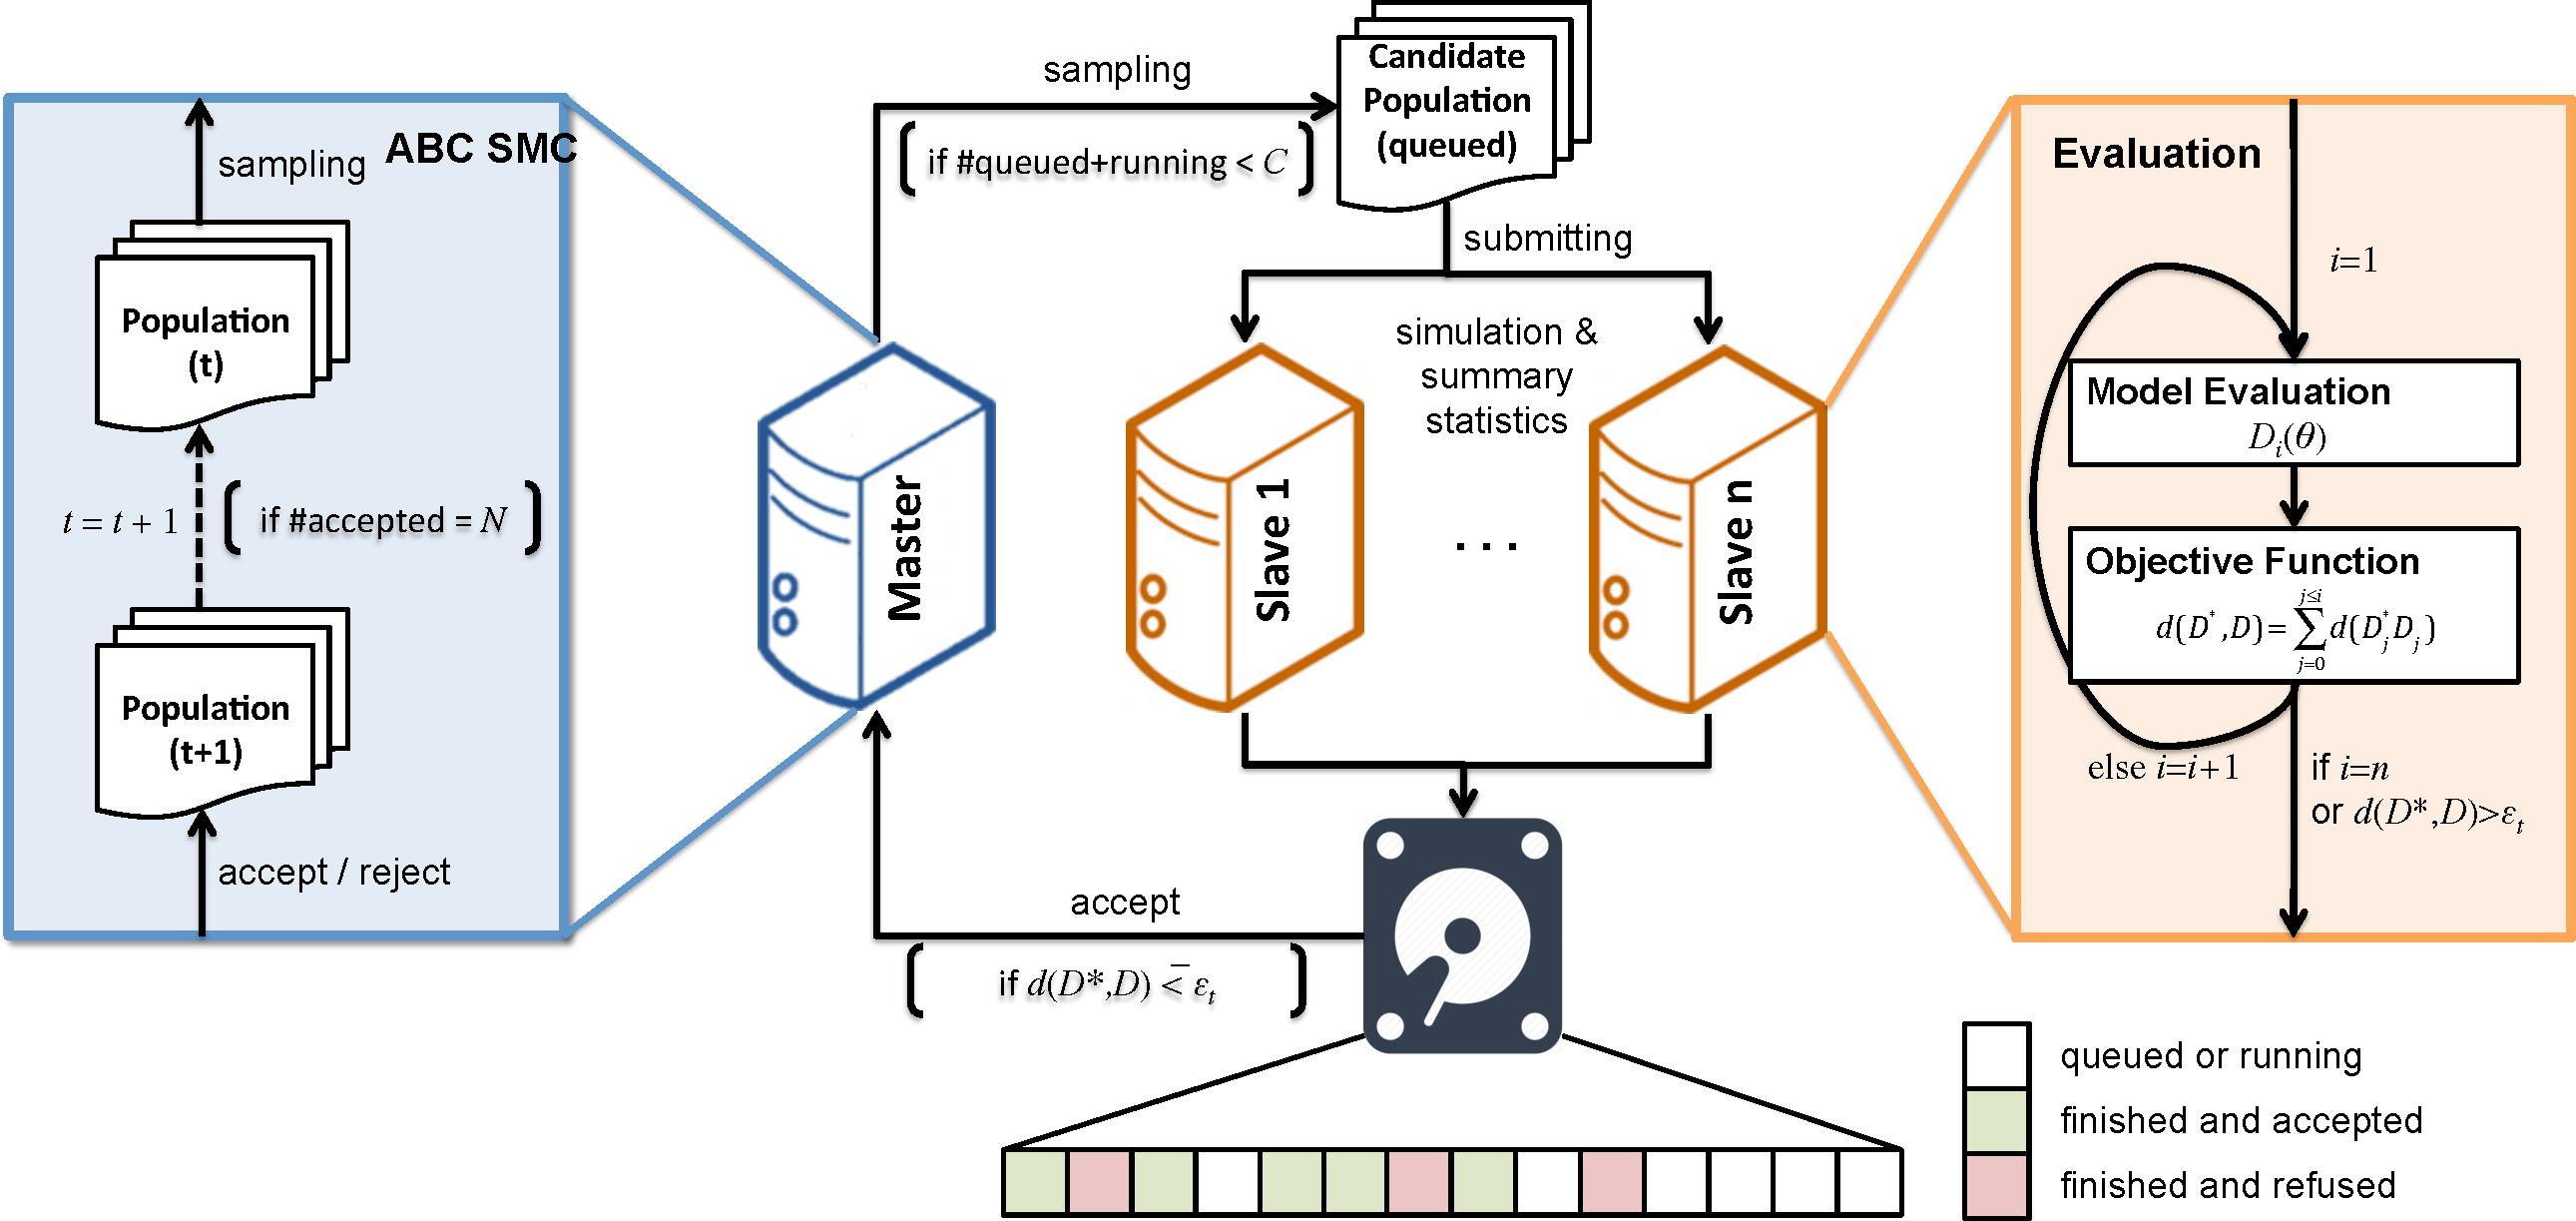
\includegraphics[width=\textwidth]{Figures/Pipeline.pdf}
\caption{{\bf Flowchart of parallel ABC~SMC methods.}
pABC~SMC uses a master/slave structure. The master performs the parameter sampling, submits the jobs, collects the results and proceeds to the next generation. Slaves simulate the model for different parameter values, evaluate the distance measure and return the results.
\jh{$\epsilon_t$!}
\jh{The simulation and objective function evaluation is actually intertwined. this is not depicted.}
\jh{We could add an illustration of ABC SMC in general.}
}
\label{fig:Pipeline}
\end{figure}

%%%%%%
%%%%%%
\subsection*{Evaluation of pABC~SMC on artificial experimental data}

To assess the properties of ABC~SMC methods for biological multi-scale process, we consider 2D and 3D models for in-vitro tumor growth we developed previously~\cite{JagiellaMul2015}. These hybrid discrete-continuum models exploit an agent-based description for individual cancer cells and a PDE-based description for extracellular metabolites and extracellular matrix components (ECM). The intracellular regulation of cell division and cell death are captured by a combination of continuous time Markov chains (CTMCs) and simple decision rules. For further details we refer to the \textit{Materials and Methods} section.

The trajectories of the tumor growth models are subject to stochastic fluctuations. In particular during the initial growth phase, which are marked by low cell numbers, stochastic simulations differ greatly. During later phases with higher cell numbers a self-averaging effect occurs. These stochastic dynamics and the multi-scale nature of the models provide an interesting but challenging inference problem.

%%%%%%
\paragraph{Artificial experimental data:}
To assess the performance of ABC SMC we created an artificial dataset for a reference parameter $\hat{\theta}$ (see Tab.~\ref{tab:model-parameters}, Scenario~I). For the parameter, cell proliferation is exclusively controlled by available space and ECM abundance. Nutritions are not limiting, which simplifies the model.

The artificial dataset closely resembles the experimental data used in later and provides growth curves and histological information. Fig.~\ref{fig2} depicts a sequence of simulation snapshots illustrating the model evolution over time and a respective experimental micrograph. The color-coding indicates that the proliferative activity is limited to an outer rim, while cells further in the interior are mostly quiescent. Because the spheroids expand outwards into zones where no ECM previously exists, one can observe a ECM gradient from the outer border toward the interior. These images provide the fraction of proliferation and relative ECM abundance and complimentary growth curves provide the time-dependent spheroid radius. All these information are in the following used for inference.

\begin{figure}[!t]
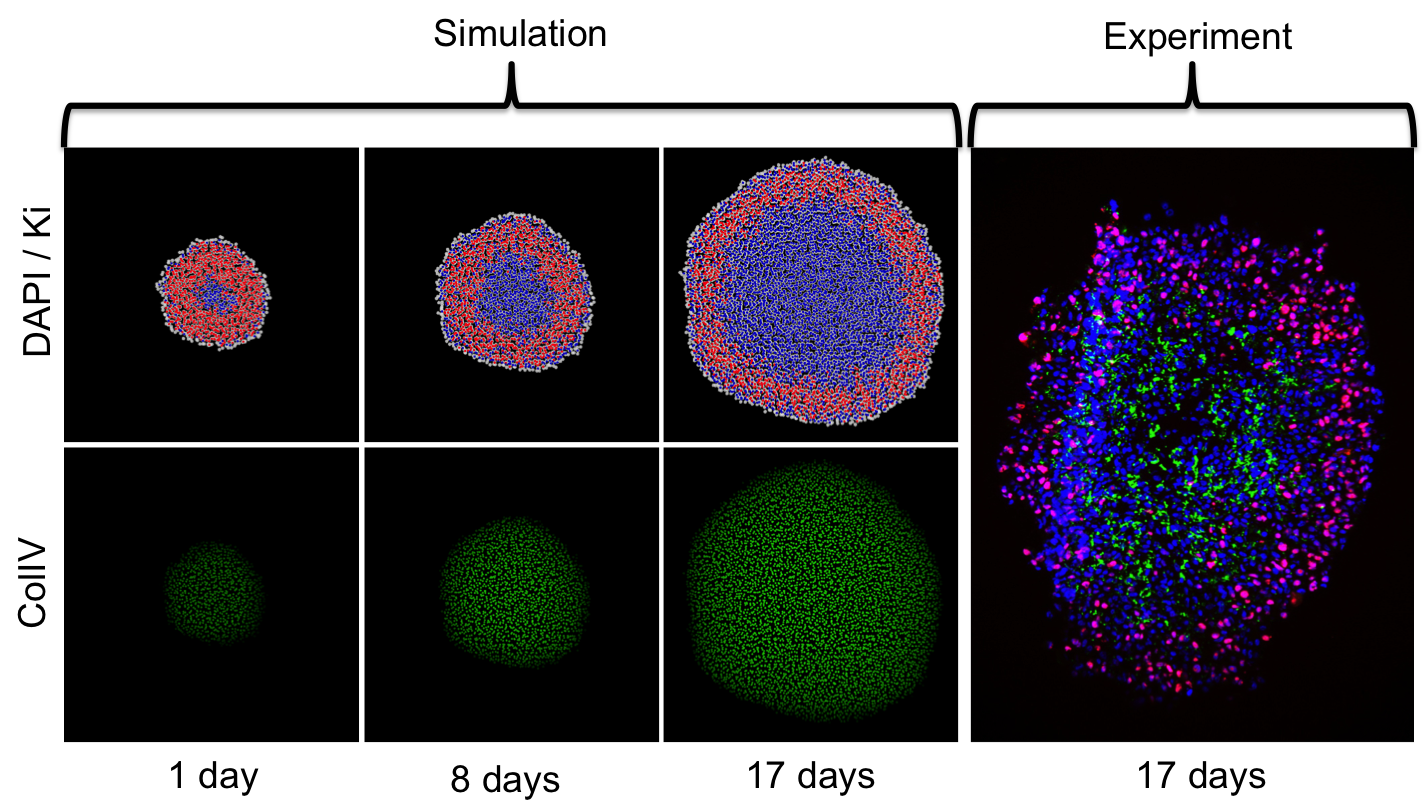
\includegraphics[width=\textwidth]{Figures/SimulationSnapshots}
\caption{{\bf Histological images of \textit{in-silicio} simulations and \textit{in-vitro} experiments.}
The cross sections depicted DAPI-stained cell nucleus (blue), Ki67-stained proliferating cells (red), and ColIV-stained extracellular matrix staining (green).}
\label{fig2}
\end{figure}

%In the following sections we present one inference run in detail and the results of a sensitivity analysis for different population sizes and additive (measurement) noise. 

%%%%%%
\paragraph{Parameter inference:}

Fig.~\ref{fig3}D shows the comparison between data and model prediction for the parameter population evolving over generations ($t=1,11,22,33,44$). One can clearly see, that the initial population spreads rather widely across the state space. With growing generations predictions resemble more and more the experimental observations for the whole population of parameters. For the final population all predicted trajectories are even mostly confined within the error bars.

As the scatter plot matrix in Fig.~\ref{fig3}C indicates, all model parameters, that were used to create the artificial data (see Tab.~\ref{tab:model-parameters}), could be identified. Nevertheless, the coupling parameter between cellular model and extracellular matrix, $e^{crit}$, needs a lot of evaluations and remains with a very large uncertainty. 

Further more, we observe, that the acceptance rate of candidate samples (Fig.~\ref{fig3}A) becomes dramatically low for objective function values small than the objective function expected at the optimum itself, $\epsilon_{t} < \epsilon_{D}$ (Fig.~\ref{fig3}B) \nj{(explain $\epsilon_{D}$ in material methods)}.

\begin{figure}[htbp]
\begin{minipage}[t]{0.33\textwidth}
%\textbf{A} \hspace{180pt} \textbf{B} \\
\textbf{A}
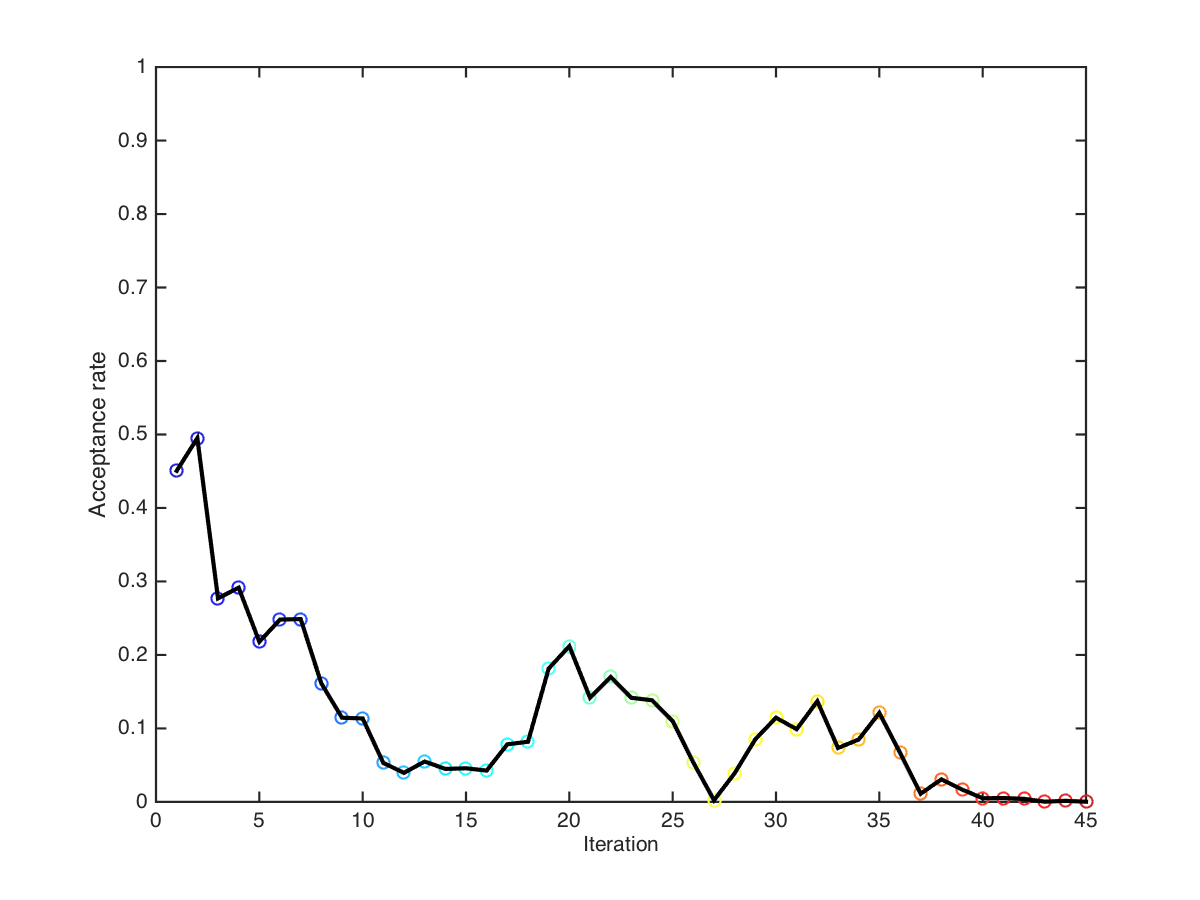
\includegraphics[width=\textwidth]{Data/TumorToyData2D_0.001merr_100pop_GCKI67ECM_NEW_acceptanceRate}\\
\textbf{B}
\includegraphics[width=\textwidth]{Data/TumorToyData2D_0.001merr_100pop_GCKI67ECM-objFunc}
\end{minipage}
\begin{minipage}[t]{0.66\textwidth}
\textbf{C}\\
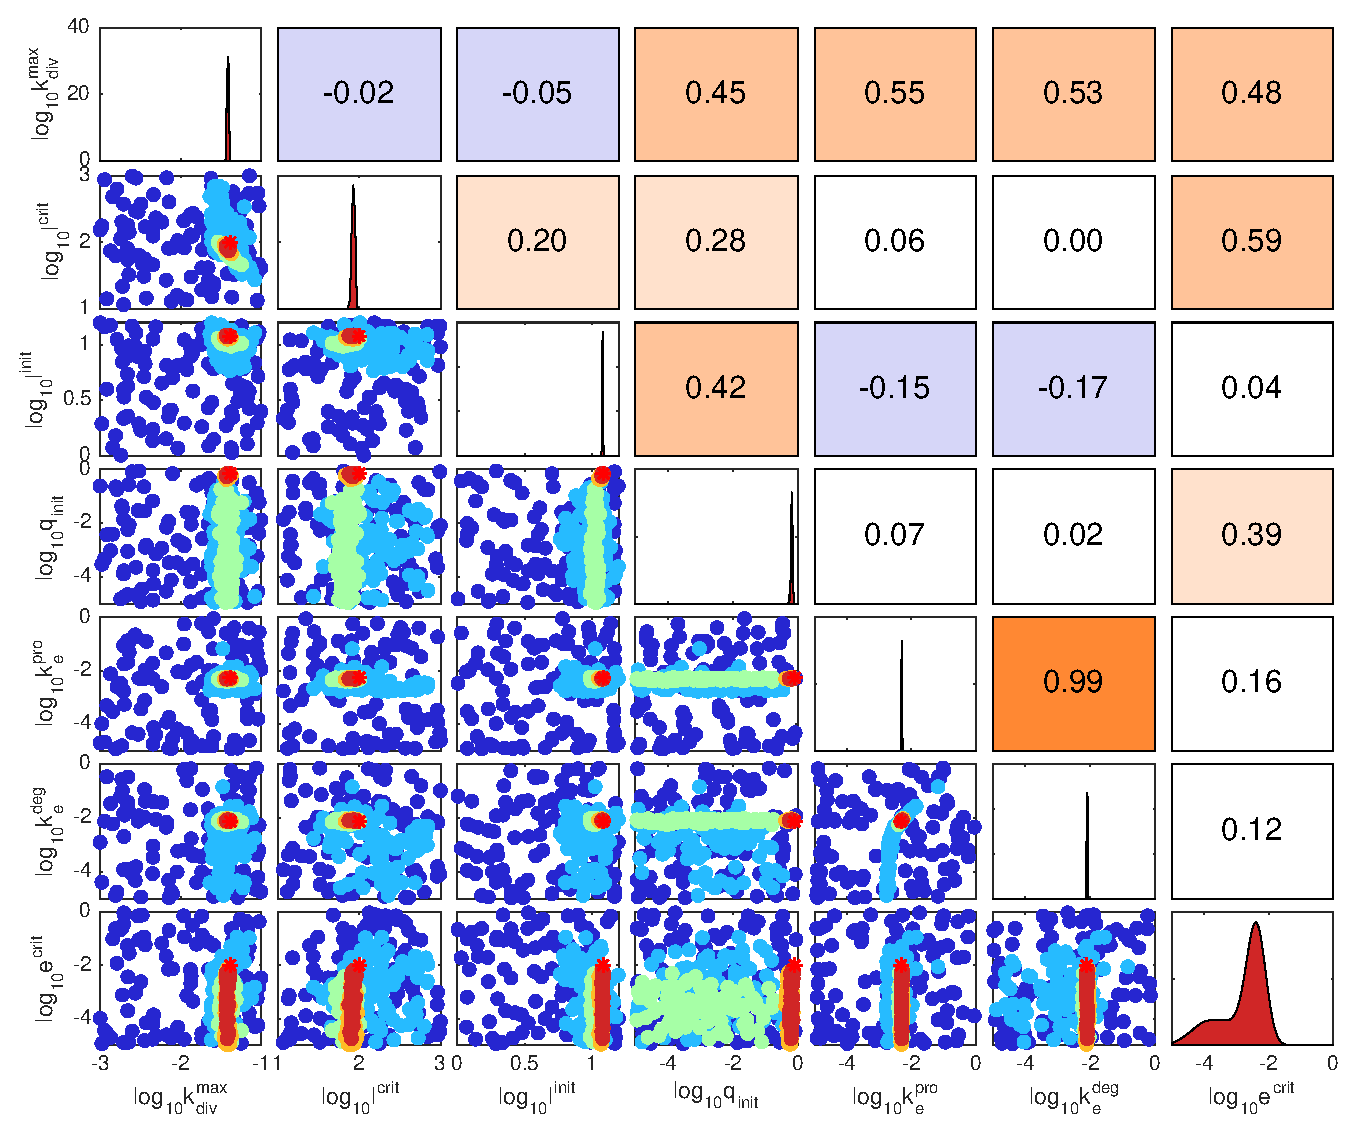
\includegraphics[width=\textwidth]{Data/TumorToyData2D_0.001merr_100pop_GCKI67ECM-scatterPlotMatrix}
\end{minipage}
\textbf{D}\\
\includegraphics[width=\textwidth]{Data/TumorToyData2D_0.001merr_100pop_GCKI67ECM-fits}
\caption{{\bf Artificial data and fits for 5 (color-coded) generation (complete dataset).}
\textbf{A}  acceptance rate over iteration; \textbf{B} $\epsilon$ threshold (cyan) and distance of the accepted population (blue) over iteration; for comparison the median distance at the optimum is depicted (red); \textbf{C} scatter matrix for 5 (color-coded) generation. todo: color spectrum. \textbf{D} Artificial data and fits for 5 (color-coded) generations (complete dataset).}
\label{fig3}
\end{figure}


%%%%%%
%%%%%%
\paragraph{Sensitivity to Population/Sample Size}
In the following we varied the population size $n$ to explore the methods sensitivity on the sample size requirement. Fig.~\ref{fig4} summarizes nicely, that the population size has in deed a critical impact on the convergence of the algorithm. If the population size is chosen too small, in our case 20, then convergence can not be assured. On the other hand, we observe no significant improvement for an increase from 100 to 200. The objective function values as well as the number of function evaluations develop similarly with increasing number of iterations. So for the means of limiting the cluster load per iteration all following parameter inference runs will be done with a population size of 100.


%%%%%%
%%%%%%
\subsection*{Experimental data (2D)} For artificial data all identifiable parameters should be inferable accurately to a certain extend depending on the model-inherent stochsticity by fitting the model to data produced by the model itself. For real data one can apriori not be sure that the model is mechanistically able to reproduce the behaviour of the biological system which lead to a data set. 

In the following we study the parameter identifiability using the same model setting I as in the previous section (see Tab.~\ref{tab:model-parameters}). The special focus lied on how the parameter va identifiability or even infered parameter values change with the amount / type of experimental data at hand. As the growth curves are the easiest information to experimentally measure compared to histological information, they will be part of all inference runs. So we test all 4 combinations of including / excluding the histological data on cell proliferation (Ki67) and extra-cellular matrix (ECM).

Fig.~\ref{fig:exp2d} 

no histological info on proliferation (Ki67) leads to wrong predictions cellular kinetic param.
kinetic ECM param. not identifiable without hist. info. on ECM (ColV)


\begin{figure}[htbp]
\textbf{A}\\
%\includegraphics[width=0.49\textwidth]{Figures/FitToyData5a}
%\includegraphics[width=0.49\textwidth]{Figures/FitToyData5b}
\includegraphics[width=\textwidth]{Data/Tumor2dGCXXXindependentBoxplots}\\
\textbf{B}\\
%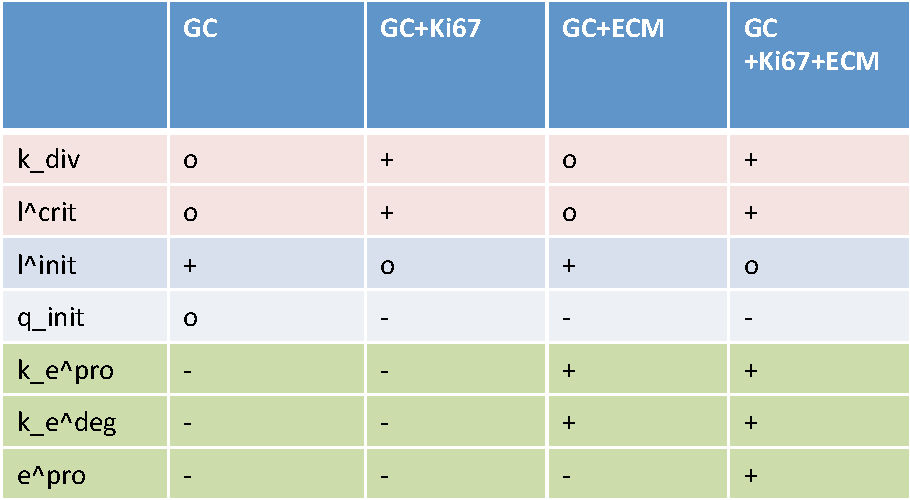
\includegraphics[width=\textwidth]{Figures/FitExpDataIdentifiabilityTable}\\
\begin{tabular}{r| r r r r }
& &KI67 &ECM &KI67ECM \\
\hline 
$k_{div}^{max}$&+ &+ &++ &+ \\
$l^{crit}$&+ &++ &+ &+ \\
$l^{init}$&++ &+ &+ &+ \\
$q_{init}$&++ &+ &+ &+ \\
$k_{e}^{pro}$&- - &- - &++ &+ \\
$k_{e}^{deg}$&- - &- - &++ &+ \\
$e^{crit}$&- - &- &- &++ \\
\end{tabular}

\begin{tabular}{r| r r r r }
& &KI67 &ECM &KI67ECM \\
\hline 
$k_{div}^{max}$& 0.815 & 0.660 & 1.000 & 0.509 \\
$l^{crit}$& 0.102 & 1.000 & 0.122 & 0.779 \\
$l^{init}$& 1.000 & 0.237 & 0.602 & 0.176 \\
$q_{init}$& 1.000 & 0.476 & 0.387 & 0.468 \\
$k_{e}^{pro}$& 0.014 & 0.019 & 1.000 & 0.260 \\
$k_{e}^{deg}$& 0.017 & 0.025 & 1.000 & 0.198 \\
$e^{crit}$& 0.046 & 0.063 & 0.081 & 1.000 \\
\end{tabular}

\textbf{C}\\
\includegraphics[width=\textwidth]{Data/Tumor2dGCXXXfit}
\caption{{\bf Different combinations of experimental data sets.}
\textbf{A} box plot for different combinations of data sets; \textbf{B} identifiablitity table (+ identifiable, o large uncertainty, - unidentifiable); \textbf{C} final fits and scenarios.}
\label{fig:exp2d}
\end{figure}

%%%%%%
%%%%%%
\subsection*{Experimental data (3D)}
Fig.~\ref{fig:exp3d} 

\begin{figure}[htbp]
\begin{minipage}[t]{0.33\textwidth}
%\textbf{A} \hspace{180pt} \textbf{B} \\
\textbf{A}
\includegraphics[width=\textwidth]{Data/Tumor3dGCKI67ECM-acceptanceRate.eps}\\
\textbf{B}
\includegraphics[width=\textwidth]{Data/Tumor3dGCKI67ECM-objFunc.eps}
\end{minipage}
\begin{minipage}[t]{0.66\textwidth}
\textbf{C}\\
\includegraphics[width=\textwidth]{Data/Tumor3dGCKI67ECM-scatterPlotMatrix.eps}
\end{minipage}
\textbf{D}\\
\includegraphics[width=\textwidth]{Data/Tumor3dGCKI67ECM-fits.eps}
\caption{{\bf Artificial data and fits for 5 (color-coded) generation (complete dataset).}
\textbf{A}  acceptance rate over iteration; \textbf{B} $\epsilon$ threshold (cyan) and distance of the accepted population (blue) over iteration; for comparison the median distance at the optimum is depicted (red); \textbf{C} scatter matrix for 5 (color-coded) generation. todo: color spectrum. \textbf{D} Artificial data and fits for 5 (color-coded) generations (complete dataset).}
\label{fig:exp3d}
\end{figure}

\begin{figure}[htbp]
\includegraphics[width=\textwidth]{Data/TumorXXXdGCKI67ECMindependentBoxplots}
\caption{{\bf Fitting experimental data: 2d versus 3d model.}
}
\label{fig:exp2dvs3d}
\end{figure}

%%%%%%
%%%%%%
\subsection*{Analysis of tumor spheroid growth using pABC~SMC}

%\begin{table}[!ht]
%\begin{adjustwidth}{-2.25in}{0in} % Comment out/remove adjustwidth environment if table fits in text column.
%\caption{
%{\bf Table caption Nulla mi mi, venenatis sed ipsum varius, volutpat euismod diam.}}
%\begin{tabular}{|l|l|l|l|l|l|l|l|}
%\hline
%\multicolumn{4}{|l|}{\bf Heading1} & \multicolumn{4}{|l|}{\bf Heading2}\\ \hline
%$cell1 row1$ & cell2 row 1 & cell3 row 1 & cell4 row 1 & cell5 row 1 & cell6 row 1 & cell7 row 1 & cell8 row 1\\ \hline
%$cell1 row2$ & cell2 row 2 & cell3 row 2 & cell4 row 2 & cell5 row 2 & cell6 row 2 & cell7 row 2 & cell8 row 2\\ \hline
%$cell1 row3$ & cell2 row 3 & cell3 row 3 & cell4 row 3 & cell5 row 3 & cell6 row 3 & cell7 row 3 & cell8 row 3\\ \hline
%\end{tabular}
%\begin{flushleft} Table notes Phasellus venenatis, tortor nec vestibulum mattis, massa tortor interdum felis, nec pellentesque metus tortor nec nisl. Ut ornare mauris tellus, vel dapibus arcu suscipit sed.
%\end{flushleft}
%\label{table1}
%\end{adjustwidth}
%\end{table}


%%%%%%
%%%%%%
%%%%%%
\section*{Discussion}

Compared to the alternative of parallelizing the model simulation directly, the suggested parallelization with respect to the drawn parameters has the advantage that the code used for model evaluation does not have to be touched. Furthermore, communication is minimized as merely the parameters and the calculated objection functions values have to be send over the network.

mention that DREAM 15 parameters, no ABC, the best performing methods applied a trick that the trick that the objective function (which is deterministic) could be optimized directly

spatial moments

Methods directly applicable to inference for models implemented in multi-scale modeling platforms such as FLAME~\cite{RichmondWal2010}, CompuCell3D~\cite{SwatTho2012}, Morpheus~\cite{StarrussBac2014}, EPISIM~\cite{SutterlinKol2013} and Chaste~\cite{MiramsArt2013}.

extension to model selection straight forward -> Toni paper
but choice of metric becomes even more important

NunesBal2010 - On optimal selection of summary statistics for approximate {B}ayesian computation 

AABC -> BuzbasRos2013

surrogates / Gaussian processes



% You may title this section "Methods" or "Models". 
% "Models" is not a valid title for PLoS ONE authors. However, PLoS ONE
% authors may use "Analysis" 
\section*{Materials and Methods}

%%%%
\subsection*{Agent-based model for tumor spheroid growth}
In this study we consider a multi-scale model describing \textit{in-vitro} tumor growth. The model exploits an individual-based description of tumor cells and a continuum-based description of key metabolites, extra-cellular matrix and waste material from cellular debris of necrotic cells. Individual cells are modeled by agents which can sense their environment, move, divide and die. Furthermore, these agents interact directly via cell-cell contract and indirectly via uptake/secretion of extracellular substances. The dynamics of extra-cellular matrix, the key metabolites and waste material are modeled using partial differential equations. The model we consider is based on own previous work \cite{JagiellaMul2015} and will be introduced in the following.
\\[2ex]
\noindent \textit{Notation:} $\Heaviside{x}$ denotes the Heaviside step function evaluate at $x$, with 
\begin{equation*}
\Heaviside{x} =  \left\{\begin{array}{ll}0 & \text{for } x < 0 \\ 1  &\text{for } x > 0. \end{array}\right.
\end{equation*}
Furthermore, we denote the second derivative with respect to space -- the Laplace operator -- by $\nabla_x$.

%%%%
\paragraph{Model for single-cell dynamics:}
Our model considers proliferating, quiescent and necrotic cells populating a static unstructured lattice. Each lattice site can be occupied by at most one cell. The behavior of a cell located at side $x$ can depend on the time-dependent local concentrations of extra-cellular matrix $e(t,x)$, glucose $g(t,x)$, oxygen $o(t,x)$, lactate $l(t,x)$, adenosine triphosphate $a(x)$ and waste material from debris of necrotic cells $w(t,x)$ as well as the distance $L(t,x)$ to the next vacant lattice side. 
\begin{itemize}
%
\item \textbf{Proliferating cells} progress in a discretized cell cycle with $m_d$ stages, $m = 1,\ldots, m_d$. The transition from stage $m$ to stage $m+1$ occurs with propensity
\begin{equation*}
k_{\text{div},m}(t,x)  = \sI{k_{\text{div}}^{\max}} m_{d} \, {\color{green} \exp\!\left[-\tfrac{L(t,x)}{\sI{L^{\text{div}}}}\right]} \!  \left(1 - \tfrac{1}{2} \Heaviside{\sII{o^{\text{div}}} - o(t,x)}\right) \! \left(1 - \tfrac{1}{2} \Heaviside{w(t,x)-\sII{w^{\text{div}}}}\right).
\end{equation*}
This transition propensity increases with the availability of oxygen and deceases in the presence of waste and with a large distance to the next vacant lattice site. As stage $m = m_g$ is reached, the cell grows and occupies an adjacent lattice side. If no adjacent lattice site is vacant, the neighing cells are pushed along the shortest path toward the closest vacant lattice site. For $m = m_{d}$, the cell divides into two daughter cells. An individual daughter cell decides to proliferate with probability
\begin{equation*}
\begin{aligned}
p_{\text{re}}(t,x) &= \exp\!\left[-\tfrac{L(t,x)}{\sI{L^{\text{div}}}}\right] \! \Heaviside{e(t,x)-\sI{e^{\text{div}}}} \Heaviside{k_a(t,x)-\sII{k_a^{\text{div}}}} \\
& \qquad \cdot \Heaviside{l(t,x)-\sII{l^{\text{div}}}} \! \Heaviside{\sII{n^{\max}} - n_{w,o}(t,x){\color{green}?}},
\end{aligned}
\end{equation*}
and becomes otherwise quiescent. Proliferating daughter cells start in the first cell cycle stage, $m = 1$. The probability to become proliferating cell depends on the local concentrations of extracellular matrix and lactate as well as on the time the cell was deprived of oxygen or exposed to waste material $n_{w,o}(x)$ and the ATP synthesis rate $k_a^{\text{div}}(t,x) = {\color{green}2 q_g(t,x) + 34 \min\{q_g(t,x),q_o(t,x)/6\}???}$. The time of oxygen deprivation and waste exposure is
\begin{equation*}
	n_{w,o}(t,x) = \int_{0}^{t}  1 -  \mathrm{H}(\sII{w^{\text{div}}}-w(\tau,x(\tau)))\mathrm{H}(o(\tau,x(\tau)) - \sII{o^{\text{div}}}) d\tau,
\end{equation*}
in which $x(\tau)$ denotes the previous locations of the cell located at $x$ at $t$. The ATP synthesis rate depends on the local glucose and oxygen consumptions, $q_g(t,x)$ and $q_o(t,x)$, which are defined below.
%
\item \textbf{Quiescent cells} are arrested in cell cycle but can reenter cell cycle and become proliferating cells with stage $m = 1$. Quiescent cell attempt to reenter the cell cycle with propensity
\begin{equation*}
	k_{\text{re}}(t,x) = \sI{k_{\text{re}}^{\max}} \left(1 - \tfrac{1}{2} \Heaviside{w(t,x)-\sII{w^{\text{div}}}}\right) \! \left(1 - \tfrac{1}{2} \Heaviside{\sII{o^{\text{div}}} - o(t,x)}\right),
\end{equation*}
and succeed with probability $p_{\text{re}}(t,x)$.
%
\item \textbf{Necrotic cells} emerge from proliferating and quiescent cells with propensity
\begin{equation*}
	k_{\text{nec}}(t,x) = \sII{k_{\text{nec}}^{\max}} \Heaviside{\sII{k_a^{\text{nec}}}-k_a(t,x)} \frac{l(t,x)^{2}}{l(t,x)^{2} + (\sII{l^{\text{nec}}})^{2}},
\end{equation*}
which at low ATP synthesis levels increases with the local lactate concentration. Necrotic cells are lysed with constant propensity $k_{\text{lys}}$ and afterwards removed from the corresponding lattice site.
\end{itemize}
The initial cell population at time point $t = 0$ occupies all lattice sites within a sphere of radius \sI{$L^{\text{init}}$} around the center of the unstructured lattice. The individual cells are quiescent with probability \sI{$q^{\text{init}}$} and proliferating (with $m=1$). 

A visual summary of all cellular processes is provided in Figure~\ref{fig:cell-states}. For a detailed discussion of the transition propensities and reentering probabilities is provided in~\cite{Jagiella2012,JagiellaMul2015}. Precise numerical values for the thresholds ($e^{\text{div}}$, $k_a^{\text{div}}$, $k_a^{\text{nec}}$, $l^{\text{div}}$, $l^{\text{nec}}$, $w^{\text{div}}$, $o^{\text{div}}$, $n^{\max}$ and $L^{\text{div}}$) at which cells change there behavior as well as the properties of the initial cell population (\sI{$L^{\text{init}}$} and \sI{$q^{\text{init}}$}) are mostly unknown. The considered parameter regimes are provided in Table~\ref{tab:model-parameters}.

%%%%
\paragraph{Model for molecular species:} 
The dynamics of the molecular species are governed by a system of partial differential equations (PDEs), accounting for different processes.
\begin{itemize}
%
\item \textbf{Glucose and oxygen}, the primary energy sources, are subject to diffusive transport and consumption,
\begin{equation*}
\begin{aligned}
	\frac{\partial g(t,x)}{\partial t} &= D_g \nabla_x g(t,x) - q_g(t,x) c(t,x), \text{ with } q_g(t,x) = V_{m,g}(t,x) \frac{g(t,x)}{g(t,x)+k_{m,g}},\\
	\frac{\partial o(t,x)}{\partial t} &= D_o \nabla_x o(t,x) - q_o(t,x) c(t,x), \text{ with } q_o(t,x) = V_{m,o}(t,x) \frac{o(t,x)}{o(t,x)+k_{m,o}}.\\
\end{aligned}
\end{equation*}
Due to the cellular metabolism the maximum consumption rates of glucose $V_{m,g}(x)$ and oxygen $V_{m,o}(x)$ is constrained by the over metabolite,
\begin{equation*}
\begin{aligned}
V_{m,g}(t,x) &= q_g^{\max} \left(1 - \left(1- \frac{q_g^{\min}}{q_g^{\max}} \right) \frac{o(t,x)}{o(t,x) + k_o} \right) \\
V_{m,o}(t,x) &= q_o^{\max} \left(1 - \left(1- \frac{q_o^{\min}}{q_o^{\max}} \right) \frac{g(t,x)}{g(t,x) + k_g} \right).
\end{aligned}
\end{equation*}
As glucose and oxygen is merely consumed by proliferating and quiescent cells, we introduce the indicator function $c(t,x)$ which is 1 if a proliferating or a quiescent cell occupies $x$ at time point $t$ and 0 otherwise. The diffusion coefficient $D_g$ and $D_o$ as well as the consumption parameters $q_g^{\min}$, $q_g^{\max}$, $k_g$, $k_{m,g}$, $q_o^{\min}$, $q_o^{\max}$, $k_o$ and $k_{m,o}$ are available from the literature (see \cite{Jagiella2012} and references therein) and listed in Table~\ref{tab:model-parameters}.

Glucose and oxygen enter the simulation domain $\Omega$ from the surrounding medium and we assume Dirichlet boundary condition, $g(t,x) = g_0$ and $o(t,x) = o_0$ for $x \in \partial\Omega$. Initially, glucose and oxygen concentrations is equivalent to this boundary conditions, $g(0,x) = g_0$ and $o(0,x) = o_0$ for $x \in \Omega$. 
%
\item \textbf{Lactate} is a by-product of the anaerobe energy metabolism. It is produced by proliferating and quiescent cells with rate $2 q_g(t,x) + 2 \min\{q_g(t,x), q_o(t,x)/6\}$ and diffuses. This leads to the model
\begin{equation*}
	\frac{\partial l(t,x)}{\partial t} = D_l \nabla_x l(t,x) + \left(2 q_g(t,x) + 2 \min\{q_g(t,x), q_o(t,x)/6\}\right) c(t,x).
\end{equation*}
We assume that lactate dilutes and zero Dirichlet boundary conditions, $l(t,x) = l_0$ for $x \in \partial\Omega$. At the state of the experiment, the lactate concentration is zero everywhere,  $l(0,x) = 0$ for $x \in \Omega$.
%
\item \textbf{Extra-cellular matrix} provides structural support for cells and is involved in cell adhesion as well as cell-to-cell communication. The components of the extra-cellular matrix are synthesized and secreted by cells and can be degraded. This yields the governing equations for the dynamics of the concentration of extra-cellular matrix,
\begin{equation*}
	\frac{\partial e(t,x)}{\partial t} = {\color{red}{k^{e}_{\text{pro}}}} c(t,x) - {\color{red}{k^{e}_{\text{deg}}}} e(t,x).
\end{equation*}
The production rate {\color{red}$k^{e}_{\text{pro}}$} and degradation rate {\color{red}$k^{e}_{\text{deg}}$} are assumed to be constant. Note that the production rate {\color{red}$k^{e}_{\text{pro}}$} as well as the division threshold {\color{red}$k^{e}_{\text{div}}$} is in units of intensity, as the absolute extracellular matrix concentration cannot be assessed experimentally.

The boundary and initial concentration of extra-cellular matrix are assumed to be zero, $e(t,x) = 0$ for $x \in \partial\Omega$ and $e(0,x) = 0$ for $x \in \Omega$.
%
\item \textbf{Waste materials} are produced by necrotic cells and degraded with a constant rate. Accordingly, the evolution equation for the waste concentration is 
\begin{equation*}
	\frac{\partial w(t,x)}{\partial t} = {\color{red}{k^{w}_{\text{pro}}}} c_{\text{nec}}(t,x) - {\color{red}{k^{w}_{\text{deg}}}} w(t,x),
\end{equation*}
with the indicator function $c_{\text{nec}}(t,x)$ being 1 if a necrotic cell occupies $x$ at time point $t$ and 0 otherwise.

As initially merely proliferation and quiescent cells are present, the initial waste concentration is zero, $w(0,x) = 0$ for $x \in \Omega$. Furthermore, as waste is not transported ad as no cells are at the boundary, we use zero Dirichlet boundary conditions, $w(t,x) = 0$ for $x \in \partial\Omega$.
\end{itemize}
A detailed list of the boundary conditions for the different scenarios and experimental conditions is provided in Table~\ref{tab:boundary conditions}.

%%%%
\paragraph{Numerical simulations:}
To simulate the individual scenarios we exploit a hybrid approach. The cellular dynamics are simulated using Gillespies algorithms~\cite{Gillespie1977}, which accounts for the stochasticity of cellular processes and decision making. The PDEs governing the spatio-temporal evolution of glucose, oxygen, lactate, extra-cellular matrix and waste concentration are discretized using finite differences and solved using an implicit scheme.
\\[1ex]
\noindent We use this hybrid simulation approach to study two scenarios:
\begin{itemize}
%
\item \textbf{Scenario 1 -- no nutrition limitation:} Glucose and oxygen are assumed to be available in excess. Hence, neither lactate nor waste material is produced. Extra-cellular matrix dynamics are sill modeled using the aforementioned PDE. To capture this scenario, different parameters are set to zero or infinity (see Table~\ref{tab:model-parameters} and~\ref{tab:boundary conditions}), effectively reducing the dimensionality of the PDE system.
%
\item \textbf{Scenario 2 -- nutrition limitation:} Glucose and oxygen are potentially limiting and all afore-described variables are simulated. We considered four experimental conditions with different glucose and oxygen concentrations (Table~\ref{tab:boundary conditions}). 
\end{itemize}
For details regarding the presented agent-based model, we refer to~\cite{Jagiella2012}.

\begin{figure}[htbp]
%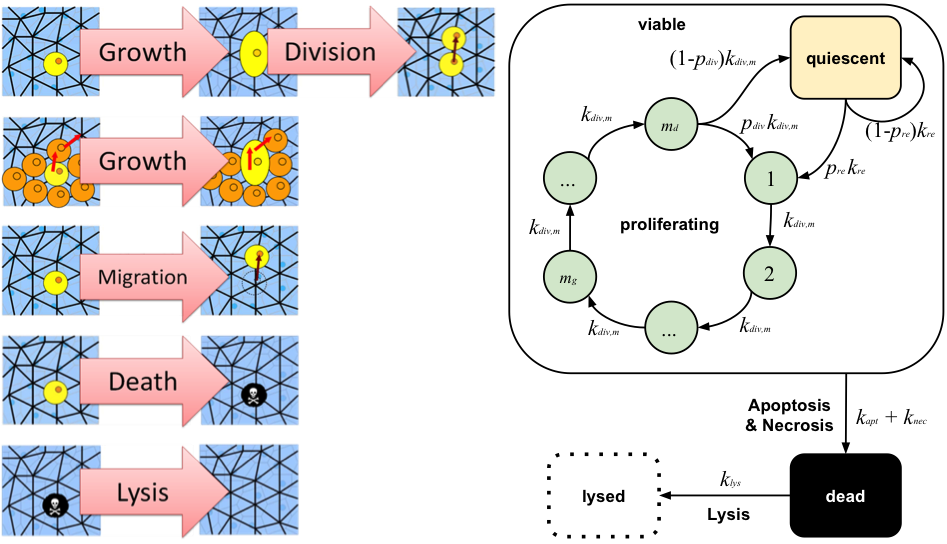
\includegraphics[width=\textwidth]{Figures/Fig5}
%\includegraphics[width=0.45\textwidth]{Figures/SpatialStateTransitions}
%\includegraphics[width=0.55\textwidth]{Figures/InternalStateTransitions}
\caption{{\bf Scheme of cell states and the biological processes a cell can undergo: cell cycle (including cell growth and division), cell death (apoptosis and necrosis) and lysis.}
 Left panel: A cycling cell grows by occupying two neighboring lattice sites after a fraction of transitions in the cell cycle. Growing cells can push a certain number of cells aside. A cell dies with rate $k_{\text{nec}}$ and is consequently lysed with rate $k_{lys}$. (The schemes in the left panel are 2D for clarity; the simulations however were all in 3D). Right: All processes are modeled as Poisson processes. A cell in the cell cycle undergoes $m_d$ transitions until splitting into two daughter cells. Composed of $m_d$ sub-processes the cell cycle time ends up following an Erlang distribution. Increasing $m_d$ will lead to sharper cell cycle distributions. A cell transitions from one cell cycle state (CCS) to the next with rate $k_{div,m}$. If a cell is in state mg it will grow. If it is in state $m_d$ it will divide into 2 daughter cells during the next transition. Furthermore, the 2 daughter cells will either enter the first CCS with probability $p_{\text{div}}$ or become quiescent (G0) with probability $1 - p_{\text{div}}$. A cell in quiescence can reenter the cell cycle with rate $k_{\text{re}}$ and probability $p_{\text{div}}$.
}
\label{fig:cell-states}
\end{figure}

\begin{table}[!ht]
\begin{adjustwidth}{-1in}{0in} % Comment out/remove adjustwidth environment if table fits in text column.
\caption{
{\bf Model parameters.} The table shows all model parameters with there respective values and ranges. For the different parameter inference settings (I: no nutriement limitation, II: nutriment limitation) the ranges for those parameters differ accordingly. For setting I some parameters were not subject to inference (*).}
\begin{tabular}{|l|r|r|r|r|r|}
\hline
\multicolumn{3}{|l|}{\bf } & \multicolumn{2}{|l|}{\bf Parameter value / range}\\ \hline
{\bf Parameter} 					&{\bf Symbol} &{\bf Unit} &\sI{\bf Scenario I} &\sII{\bf Scenario II}\\ \hline
division rate 					&$k_{\text{div}}^{\max}$ & 1/h & 0.032 & $0.032 \times 10^{-2...2}$\\ \hline
division depth 					&$L^{\text{div}}$ & $\mu$m & 130 & 1.3...13000\\ \hline
initial population radius 			&$L^{\text{init}}$ & $\mu$m & 130 & 0.12...1200\\ \hline
initial quiescent cell fraction 		& $q{\text{init}}$ &-& 0.75& 0.0075...75\\ \hline
ECM production rate 			&$k_{e}^{\text{pro}}$  & {\color{green}UI}/h&0.0005 &0.000005...0.05\\ \hline
ECM degradation rate 			&$k_{e}^{\text{deg}}$ &1/h&0.0033 &0.000033...0.33\\ \hline
ECM division threshold 			&$e^{\text{div}}$ &{\color{green}UI} &0.003 &0.00003...0.3\\ \hline
\hline
cell cycle reentrance rate 			&$k^{\max}_{\text{re}}$ &1/h &0*{\color{green}??}&0.00001...0.1\\ \hline
necrosis rate 					&$k_{\text{nec}}$ &1/h&0*&0.0001...1\\ \hline
lysis rate 						&$k_{\text{lys}}$ &1/h&0*&0.0001...1\\ \hline
ATP synthesis division threshold 			&$k_a^{\text{div}}$ &mM/h& 0*& 9...90000\\ \hline
ATP synthesis necrosis threshold 			&$k_a^{\text{nec}}$ &mM/h& 0*& 6...60000\\ \hline
lactate division threshold 			&$l^{\text{div}}$  &mM&$\infty$* & 0.2...2000\\ \hline
lactate necrosis threshold 			&$l^{\text{nec}}$ &mM &$\infty$* & 0.2...2000\\ \hline
{\color{green}oxygen diffusion coefficient?} 			&$D_o$&  &  &  \\ \hline
{\color{green}glucose diffusion coefficient?} 			&$D_g$&  &  &  \\ \hline
waste diffusion coefficient 			&$D_W$& $\mu$m$^{2}$/h&$\infty$*& $10^{3}...10^{7}$\\ \hline
waste degradation rate					& $k^w_{\text{deg}}$ &1/h &$0$*& $10^{-8}...10^{-4}$\\ \hline
waste division threshold 			&$w^{\text{div}}$ &{\color{green}mM} &$\infty$*&0.00008...0.8\\ \hline
waste exposure cell cycle threshold {\color{green}oxygen?} 	&$n_{o,w}$&{\color{green}mM}& $\infty$*& 0.08...800\\ \hline
\end{tabular}
\label{tab:model-parameters}
\end{adjustwidth}
\end{table}



%\paragraph{Molecular model:} The molecular dynamics is described by system of partial differential equations as follows:
%\begin{align}
%	\partial_{t} e &= {\color{red}{k^{e}_{pro}}} c - {\color{red}{k^{e}_{deg}}} e,\\
%	\partial_{t} g &= D \nabla g - k^{g}_{con} c,\\
%	\partial_{t} o &= D \nabla o - k^{o}_{con} c,\\
%	\partial_{t} a &=k^{a}_{pro}c - k^{a}_{con} c, k^{a}_{pro} =  2k^{g}_{con} c + 17/3 k^{o}_{con},\\
%	\partial_{t} w &= {\color{red}{k^{w}_{pro}}} c_{nec} - {\color{red}{k^{w}_{deg}}} w,\\
%\end{align}
%where $c=1$, if the a living cell is occupying the volume, or $c_{nec}=1$, if a necrotic cell is occupying the same volume. Else $c=c_{nec}=0$.
%
%consumption rates
%
%\paragraph{Initial \& boundary conditions:}
%The initial cell population occupies all lattice sites within a sphere of radius {\color{red}{$l^{init}$}}. A fraction of those cells $\color{red}{q_{init}}$ is quiescent right from the start, while the rest enters the cell cycle with $M=1$. For the molecular concentration we assume Dirichelet boundary conditions. That is to say, that molecular concentrations at the boundary of the domain $\partial \Omega$ are kept constant (see table \ref{tab:boundary conditions}).
%
%\paragraph{Numerical simulations:}
%The cellular dynamics is treated like a chemical reaction system were each cell and the biological process it can perform can be seen as analogues to a chemical species and reactions. As such one can formulate a master equation and solve it numerically using the Gillespie algorithm \nj{[ref]}.  


\begin{table}[!ht]
\begin{adjustwidth}{-0.5in}{0in} % Comment out/remove adjustwidth environment if table fits in text column.
\caption{
{\bf Boundary conditions.}}
\begin{tabular}{|l |r |r|r|r|r|}
\hline
 			& {\bf Scenario I} & \multicolumn{4}{|c|}{\bf Scenario II}\\ \hline
{\bf Molecule} 	&				&{\bf Condition I} 	&{\bf Condition II} 	&{\bf Condition III} 	&{\bf Condition IV}\\ \hline
$g$			& * 				& $1$ mM			& $5$ mM			& $25$ mM			&$25$ mM\\ \hline
$o$			& *				& $0.28$ mM		& $0.28$ mM		& $0.28$ mM			&$0.07$ mM\\ \hline
$l$				& *				& $0$ mM			& $0$ mM			& $0$ mM				& $0$ mM\\ \hline
$e$			& $0$ mM		& $0$ mM			& $0$ mM			& $0$ mM				& $0$ mM\\ \hline
$w$			& $0$ mM		& $0$ mM			& $0$ mM			& $0$ mM				& $0$ mM\\ \hline
\end{tabular}
For setting I some molecule dynamics were not considered (*).
\label{tab:boundary conditions}
\end{adjustwidth}
\end{table}

%%%%
%%%%
\subsection*{Experimental Data}
In this study we considered two data types: growth curves and histological imaging data. Growth curves provide the measured radius of spheroids $r^m(t_k)$ at time points $t_1, \ldots, t_{n_g}$. Histological imaging data provide the fraction of proliferating cells $f^m(t_k,d_l)$ and the extracellular matrix distribution $e^m(t_k,d_l)$ at distances $d_1, \ldots d_{n_d}$ from the spheroid border and time points $t_1, \ldots, t_{n_h}$. The experimental data were collected under up to four experimental conditions with different glucose and oxygen concentrations and processed by Jagiella et al. \cite{JagiellaMul2015}. For further details we refer to the original publication.

%%%%
%%%%
\subsection*{Parallel ABC~SMC}
For this study we developed a simple parallelized version of the ABC SMC method introduced by Toni et al.~\cite{ToniWel2009}. The master node runs the main routine which iteratively samples $T$ generations, $t = 0$ to $t = T-1$, with decreasing tolerances, $\epsilon_0>\ldots>\epsilon_{T-1}$. To explore several cores, candidate parameters are evaluated in parallel. To ensure convergence of the sampling to the true posterior, the main routing keeps track of the order of the candidate parameters. Merely if the evaluation for the candidate parameters $j = 1,\ldots,J$ is finished and if these candidate parameters resulted in $N$ accepted points, the algorithm continuous with the next generation. The pseudocode of the main routine is:
% Parallel ABC SMC
\paragraph{Main routine: Parallel ABC~SMC}
\begin{itemize}
\item[\it In:]
Number of generations $T$, number of samples per generation $N$ and number of available cores $C$.
%
\item[\it S1]
Set the generation indicator $t=0$. \\
Set the initial threshold $\epsilon_{0} = \infty$.\\
%
\item[\it S2] Set the candidate number $j = 1$.
\item[\it S3] If number of jobs on queue is below or drops below $C$, determine from stored files the smallest candidate number $J+1$ for which no results are available.
	\begin{itemize}
	\item[$\bullet$] If number of accepted candidates in the set $j = 1,\ldots,J$ is $N$, assign parameters and normalized weights to $\{\theta^{(i)}_{t-1}\}_{i=1}^N$ and $\{w^{(i)}_{t-1}\}_{i=1}^N$.
	\item[$\bullet$] Else, start new job on computing cluster by executing the subroutine $\mathrm{getSample}\!\left(t,\epsilon_t,j,\{\theta^{(i)}_{t-1}\}_{i=1}^N,\{w^{(i)}_{t-1}\}_{i=1}^N\right)$, set $j = j +1$ and go to S3.
	\end{itemize}
\item[\it S4] If $t < T$ set $t = t+1$, $\epsilon_t = f(\{d^{(i)}\}_{i=1}^N)$ and go to S2. \\
Else, stop algorithm and output results.
\item[\it Out:] Samples $\{\theta^{(i)}_{t}\}_{i=1}^N$ and weights $w^{(i)}_{t}$.
\end{itemize}
%
The main routine calls a subroutine which runs on a slave and initiates an individual sample. In generation $t$ a sample from generation $t-1$ is selected and perturbed using the perturbation kernel $K_t(\theta|\theta')$ to obtain a new candidate parameter. If a stochastic simulation using this candidate parameters yields a distance $d$ between simulation and data below the tolerance $\epsilon_t$, this candidate is accepted. Otherwise, it is rejected. The pseudocode for this subroutine is:
%
\paragraph{Subroutine: Sampling and evaluation of candidate parameter, $\boldsymbol{\mathrm{getSample}(\cdot)}$}
\begin{itemize}
%
\item[\it In:]
Generation number $t$, tolerance $\epsilon_t$, candidate number $j$, sample $\{\theta^{(i)}_{t-1}\}_{i=1}^N$ and weights $\{w^{(i)}_{t-1}\}_{i=1}^N$ from previous generation.
%
\item[\it S1] If $t=0$, sample candidate parameter $\theta^*$ independently from the prior, $\theta^* \sim p(\theta)$. \\
Else, sample $\theta'$ from the previous generation $\{\theta^{(i)}_{t-1}\}_{i=1}^I$ with probability $w^{(i)}_{t-1}$ and perturb it to obtain the candidate parameter $\theta^* \sim K_t(\theta|\theta')$. If prior probability of $\theta^*$ is zero, $p(\theta^*) = 0$, return to S1.
\item[\it S2] Sample candidate dataset $\mathcal{D}^*$ by simulating the model, $\mathcal{D}^* \sim p(\mathcal{D}|\theta^*)$.
\item[\it S3] Create a file indicating the generation and candidate number, $t$ and $j$, and write the parameter candidate $\theta^*$, distance $d(\mathcal{D}^*,\mathcal{D},\infty)$ and weight 
\begin{equation*}
w_t^{(i)} = \left\{\begin{array}{ll}
1 &, \text{if } t = 0 \\
\dfrac{p(\theta^*)}{\sum_{j=1}^{N} w_{t-1} K_t(\theta^{(j)}_{t-1}|\theta^*)} &, \text{otherwise},
\end{array}\right.
\end{equation*}
in the created file.
\end{itemize}
%
In order to increase computational efficiency, we use a sophisticated implementation which stops the model simulation in step \textit{S2} as soon as the tolerance $\epsilon_t$ is reached. In this case, $d(\mathcal{D}^*,\mathcal{D},\infty) > \epsilon_t$ is returned. This is possible as we use a distance $d(\mathcal{D}^*,\mathcal{D},t_{\text{sim}})$ which is monotonically increases in the simulation time $t_{\text{sim}}$.

%
\paragraph{Distance measure:}
Our statistical analysis indicated a multiplicative error. For this reason, we use as distance the sum of weighted least squares,
\begin{equation*}
\begin{aligned}
d(\mathcal{D}^*,\mathcal{D},t_{\text{sim}}) 
&= \frac{1}{n_g}\sum_{k=1}^{n_g} \Heaviside{t_{\text{sim}} - t_k} \! \left(\frac{r^m(t_k) - r(t_k,\theta^*)}{\bar{r}^m}\right)^2 \\
&+ \frac{1}{n_h n_d}\sum_{k=1}^{n_h} \Heaviside{t_{\text{sim}} - t_k} \sum_{l=1}^{n_d} \left(\frac{f^m(t_k,d_l) - f(t_k,d_l,\theta^*)}{\bar{f}^m}\right)^2 \\
&+ \frac{1}{n_h n_d} \sum_{k=1}^{n_h} \Heaviside{t_{\text{sim}} - t_k} \sum_{l=1}^{n_d} \left(\frac{e^m(t_k,d_l) - e(t_k,d_l,\theta^*)}{\bar{e}^m}\right)^2.
\end{aligned}
\end{equation*}
with average values of the measured quantities
\begin{equation*}
\bar{r}^m = \sum_{k=1}^{n_g} r^m(t_k), \quad
\bar{f}^m = \sum_{k=1}^{n_h} \sum_{l=1}^{n_d} f^m(t_k,d_l) \quad \text{and} \quad
\bar{e}^m = \sum_{k=1}^{n_h} \sum_{l=1}^{n_d} e^m(t_k,d_l).
\end{equation*}
The first term penalizes the relative error in the spheroid radius, the second term the relative error in the fraction of proliferation cells and the third term the relative errors in the extracellular matrix density. All contributions are normalized with the corresponding number of measurements. As the simulation is run till time point $t_{\text{sim}}$, merely measurements with $t_k \leq t_{\text{sim}}$ are considered. For $t_{\text{sim}} > \max\{t_{n_g},t_{n_h}\}$, all measurement data are considered. This final distance is denoted by $d(\mathcal{D}^*,\mathcal{D},\infty)$.

In Section {\color{green}?}, several experimental conditions are considered simultaneously. In this case, the overall distance $d$ is the sum of the distances for the individual conditions.

%
\paragraph{Adaptation of perturbation kernel and tolerance:}
The efficiency of ABC~SMC methods depends critically on the perturbation kernels~\cite{FilippiBar2013} and the tolerance sequence~{\color{green}cite?}. To facilitate the applicability of the algorithms to a wide range of inference problems, we implemented adaptive methods. Inspired by kernel density estimation~\cite{Scott1992}, a multi-variate normal distribution is used as perturbation kernel,
\begin{equation*}
K_t(\theta|\theta') = \mathcal{N}(\theta|\theta',\Sigma_{t-1}),
\end{equation*}
with $\Sigma_t$ being the {\color{green}scaled????} covariance matrix of sample $\{\theta^{(i)}_{t-1}\}_{i=1}^N$. This perturbation kernel adapts to the correlation structure of the sample, thereby improving the representation of the distribution. The tolerance for generation $t$ is set to the median of the accepted distances in generation $t-1$.

%% Standard ABC SMC
%\paragraph{Algorithm~0: ABC~SMC}
%\begin{itemize}
%%
%\item[\it Input:]
%Number of samples per generation $N$ and number of cores one queue $C$.
%%
%\item[\it S1]
%Set the generation indicator $t=0$. \\
%Set the initial threshold $\epsilon_{0} = \infty$.\\
%%
%\item[\it S2.0] Set the particle indicator $i = 1$.
%\item[\it S2.1] If $t=0$, sample candidate parameter $\theta^*$ independently from the prior, $\theta^* \sim p(\theta)$. \\
%Else, sample $\theta'$ from the previous generation $\{\theta^{(i)}_{t-1}\}_{i=1}^I$ with probability $w^{(i)}_{t-1}$ and perturb it to obtain the candidate parameter $\theta^* \sim K_t(\theta|\theta')$. If $p(\theta^*) = 0$ return to S2.1.
%\item[\it S2.2] Sample candidate dataset $\mathcal{D}^*$ by simulating the model, $\mathcal{D}^* \sim p(\mathcal{D}|\theta^*)$.
%\item[\it S2.3] If $d(\mathcal{D}^*,\mathcal{D}) > \epsilon_t$, go to S2.1. \\
%Else, set $\theta^{(i)} = \theta^*$, $d^{(i)} = d(\mathcal{D}^*,\mathcal{D})$ and 
%\begin{equation*}
%w_t^{(i)} = \left\{\begin{array}{ll}
%1 &, \text{if } t = 0 \\
%\dfrac{p(\theta^*)}{\sum_{j=1}^{N} w_{t-1} K_t(\theta^{(j)}_{t-1}|\theta^{(i)}_{t})} &, \text{otherwise}.
%\end{array}\right.
%\end{equation*}
%\item[\it S2.3]  If $i < N$, set $i = i + 1$, go to S2.1. \\
%Else, normalize weighs $w_t^{(i)} = w_t^{(i)}/(\sum_{j=1}^N w_t^{(j)})$.
%\item[\it S3] If $t < T$ set $t = t+1$, $\epsilon_t = f(\{d^{(i)}\}_{i=1}^N)$ and go to S2.0. \\
%Else, stop algorithm and output results.
%\item[\it Output:] Samples $\{\theta^{(i)}_{t-1}\}_{i=1}^N$ and weights $w^{(i)}_{t-1}$.
%\end{itemize}

%%%%
%%%%
\subsection*{Implementation}
The agent-based model for tumor spheroid growth is implemented in C++. For parallel ABC~SMC algorithm and the evaluation of the results is implemented in MATLAB. The code for the simulation and inference is available in the GitHub repository {\color{green}...}. 

%%%%%%
%%%%%%
%%%%%%
\section*{Supporting Information}

\begin{figure}[p]
\textbf{A} \hspace{180pt} \textbf{B} \\
\includegraphics[width=0.49\textwidth]{Data/TumorToyData2D_0.001merr_XXX0pop_GCKI67ECMfunctionEvaluations}
\includegraphics[width=0.49\textwidth]{Data/TumorToyData2D_0.001merr_XXX0pop_GCKI67ECMobjectiveFunction}\\
 \textbf{C} \\
\includegraphics[width=\textwidth]{Data/TumorToyData2D_0.001merr_XXX0pop_GCKI67ECMindependentBoxplots}\\
 \textbf{D} \\
\includegraphics[width=\textwidth]{Data/TumorToyData2D_0.001merr_XXX0pop_GCKI67ECMfit}\\
\caption{{\bf Sensitivity to Population/Sample Size.}
\textbf{A}  number of function evaluations over iteration; \textbf{B} threshold over iteration; \textbf{C} box plot of final sample for different population sizes. \textbf{D} final fits.}
\label{fig4}
\end{figure}

% Include only the SI item label in the subsection heading. Use the \nameref{label} command to cite SI items in the text.
%\subsection*{S1 Video}
%\label{S1_Video}
%{\bf Bold the first sentence.}  Maecenas convallis mauris sit amet sem ultrices gravida. Etiam eget sapien nibh. Sed ac ipsum eget enim egestas ullamcorper nec euismod ligula. Curabitur fringilla pulvinar lectus consectetur pellentesque.
%
%\subsection*{S1 Text}
%\label{S1_Text}
%{\bf Lorem Ipsum.} Maecenas convallis mauris sit amet sem ultrices gravida. Etiam eget sapien nibh. Sed ac ipsum eget enim egestas ullamcorper nec euismod ligula. Curabitur fringilla pulvinar lectus consectetur pellentesque.
%
%\subsection*{S1 Fig}
%\label{S1_Fig}
%{\bf Lorem Ipsum.} Maecenas convallis mauris sit amet sem ultrices gravida. Etiam eget sapien nibh. Sed ac ipsum eget enim egestas ullamcorper nec euismod ligula. Curabitur fringilla pulvinar lectus consectetur pellentesque.
%
%\subsection*{S2 Fig}
%\label{S2_Fig}
%{\bf Lorem Ipsum.} Maecenas convallis mauris sit amet sem ultrices gravida. Etiam eget sapien nibh. Sed ac ipsum eget enim egestas ullamcorper nec euismod ligula. Curabitur fringilla pulvinar lectus consectetur pellentesque.
%
%\subsection*{S1 Table}
%\label{S1_Table}
%{\bf Lorem Ipsum.} Maecenas convallis mauris sit amet sem ultrices gravida. Etiam eget sapien nibh. Sed ac ipsum eget enim egestas ullamcorper nec euismod ligula. Curabitur fringilla pulvinar lectus consectetur pellentesque.

%%%%%%
%%%%%%
%%%%%%
\section*{Acknowledgements}

%(this will go in the funding statement provided in the online submission system)

The authors acknowledge financial support from the German Federal Ministry of Education and Research (BMBF) within the SYS-Stomach project (Grant No. 01ZX1310B), the European Union within the ERC grant ``LatentCauses'', and the Postdoctoral Fellowship Program (PFP) of the Helmholtz Zentrum M\"unchen.

%%%%%%
%%%%%%
%%%%%%
\section*{Author Contributions}

Conceived and Designed the Methods: NJ DR FJT JH.
Developed Models: NJ.
Performed Numerical Experiments: NJ DR.
Wrote the Paper: NJ JH.

\nolinenumbers

%%%%%%
%%%%%%
%%%%%%
\bibliography{Database}


\end{document}

